% ===========================================================================
%  EDA piloto — ¿En qué minuto se perdió la partida?
%  Héctor Manuel Morán Maldonado
%  Compilar:  latexmk -pdf lol_eda.tex
% ===========================================================================
\documentclass[11pt,letterpaper]{article}

\usepackage[utf8]{inputenc}
\usepackage[T1]{fontenc}
\usepackage[spanish,es-tabla,es-nodecimaldot]{babel}
\usepackage{lmodern}
\usepackage{microtype}
\usepackage[margin=2.5cm,top=2.6cm,bottom=2.6cm]{geometry}
\usepackage{graphicx}
\usepackage{booktabs}
\usepackage{longtable}
\usepackage{array}
\usepackage{float}
\usepackage{xcolor}
\usepackage{amsmath}
\usepackage{enumitem}
\usepackage{caption}
\usepackage{fancyhdr}
\usepackage{titlesec}
\usepackage[hidelinks]{hyperref}

\definecolor{azul}{HTML}{2A78D6}
\definecolor{naranja}{HTML}{EB6834}
\definecolor{aqua}{HTML}{1BAF7A}
\definecolor{tinta}{HTML}{1A1A19}
\definecolor{suave}{HTML}{52514E}
\definecolor{papel}{HTML}{F4F6F8}

\captionsetup{font=small,labelfont={bf,color=azul},width=.92\linewidth}
\titleformat{\section}{\Large\bfseries\color{tinta}}{\thesection}{.7em}{}
\titleformat{\subsection}{\large\bfseries\color{suave}}{\thesubsection}{.7em}{}
\titlespacing*{\section}{0pt}{2.2ex plus 1ex minus .2ex}{1.2ex plus .2ex}

\pagestyle{fancy}\fancyhf{}
\renewcommand{\headrulewidth}{.4pt}
\fancyhead[L]{\footnotesize\color{suave}EDA piloto · ¿En qué minuto se perdió la partida?}
\fancyhead[R]{\footnotesize\color{suave}H. M. Morán Maldonado}
\fancyfoot[C]{\footnotesize\color{suave}\thepage}

\newsavebox{\cajaresp}
\newenvironment{respuesta}[1]
  {\par\medskip\setlength{\fboxsep}{10pt}%
   \begin{lrbox}{\cajaresp}%
   \begin{minipage}{\dimexpr\linewidth-2\fboxsep-3pt\relax}%
   \color{tinta}\textcolor{azul}{\textbf{#1}}\par\smallskip\ignorespaces}
  {\end{minipage}%
   \end{lrbox}%
   \noindent\textcolor{azul}{\rule[-\dp\cajaresp]{3pt}{\dimexpr\ht\cajaresp+\dp\cajaresp\relax}}%
   \colorbox{papel}{\usebox{\cajaresp}}\par\medskip}

\newcommand{\dato}[1]{\textbf{\textcolor{azul}{#1}}}

\begin{document}

% ===========================================================================
\begin{titlepage}
\thispagestyle{empty}
\centering
\vspace*{0.6cm}

\includegraphics[width=6.4cm]{assets/logo-up.png}

\vspace{1.1cm}
{\large\color{suave}Especialidad en Ciencia de Datos\par}
\vspace{0.25cm}
{\large\color{suave}Visualización de datos y narración de historias\par}

\vspace{1.5cm}
{\color{azul}\rule{\linewidth}{1.6pt}}
\vspace{0.85cm}

{\Huge\bfseries El contexto lo cambia todo\par}
\vspace{0.45cm}
{\LARGE Análisis exploratorio piloto del corpus\\[.25cm]
 \emph{¿En qué minuto se perdió la partida?}\par}
\vspace{0.35cm}
{\large\color{suave} Datos de la API de Riot Games\par}

\vspace{0.85cm}
{\color{azul}\rule{\linewidth}{1.6pt}}

\vfill

\begin{minipage}{0.46\linewidth}
  \raggedright
  {\color{suave}\small ALUMNO}\par\smallskip
  {\large Héctor Manuel Morán Maldonado\par}
\end{minipage}\hfill
\begin{minipage}{0.46\linewidth}
  \raggedleft
  {\color{suave}\small PROFESOR}\par\smallskip
  {\large Dr.\ Rodolfo Rubén Álvarez González\par}
\end{minipage}

\vspace{1.1cm}
{\color{suave}\rule{\linewidth}{.4pt}}
\vspace{0.45cm}

{\color{suave}\small
7 partidas · 68 participantes · 2\,054 cuadros-jugador · 6\,877 eventos\\
Todas las cifras se calcularon directamente de los JSON crudos\par}

\vspace{0.55cm}
{\color{suave} \today}
\end{titlepage}

\tableofcontents
\newpage

% ===========================================================================
\section{Contexto: qué es este corpus y qué no es}

Este documento explora el conjunto de datos del proyecto \emph{¿En qué minuto se
perdió la partida?}, cuyo objetivo es reconstruir partidas de League of Legends
minuto a minuto para identificar cuándo cambia su dirección.

\begin{respuesta}{Advertencia de alcance, antes que cualquier número}
Las \dato{7 partidas} de este corpus \textbf{no son mías}. Son ejemplos públicos
del repositorio de esquemas de la API de Riot, y sirvieron para probar el canal de
datos \emph{antes} de tener una llave. Por eso todo lo que sigue describe la
\textbf{estructura del dato y el método}, nunca el desempeño de un jugador.
Con siete partidas no se puede afirmar nada sobre League of Legends ni sobre mí.
\end{respuesta}

\subsection{Las fuentes}
\begin{itemize}[leftmargin=1.4em,itemsep=.25em]
  \item \textbf{Riot Games API}, endpoint \texttt{match-v5}. Por cada partida
        entrega dos documentos: el \emph{registro} (resultado, campeones, roles,
        estadísticas finales) y la \emph{línea temporal} (el estado del juego
        cuadro por cuadro, más la lista de eventos).
  \item \textbf{Data Dragon}, CDN estático y sin llave, para traducir
        identificadores a nombres e imágenes.
\end{itemize}

\subsection{Cuatro granos, no una tabla}
Ésta es la diferencia más importante frente a un archivo como el Titanic: no hay
un solo CSV con una fila por observación. El dato llega en JSON anidado, y de él
se derivan cuatro tablas de granos distintos:

\begin{table}[H]\centering\small
\caption{Los cuatro granos derivados del JSON, y qué es una fila en cada uno.}
\label{tab:granos}
\begin{tabular}{llrl}
\toprule
Tabla & Una fila es & Filas & Variable típica \\
\midrule
\texttt{partidas} & una partida & 7 & duración, cola, parche \\
\texttt{participantes} & un jugador en una partida & 68 & oro, daño, KDA, rol \\
\texttt{cuadros} & un jugador en un minuto & 2\,054 & oro acumulado, posición \\
\texttt{eventos} & un suceso con marca de tiempo & 6\,877 & tipo, minuto, equipo \\
\bottomrule
\end{tabular}
\end{table}

\noindent La pregunta del proyecto vive en el tercer y cuarto grano: la ventaja de
oro por minuto se construye agregando \texttt{cuadros}, y el «punto de quiebre» se
busca cruzándola con \texttt{eventos}.

% ===========================================================================
\section{Calidad de datos}

\begin{table}[H]
\centering
\small
\caption{Las siete partidas del corpus. Una no es 5v5.}
\label{tab:corpus}
\begin{tabular}{lrrrrrr}
\toprule
matchId & parche & cola & jugadores & duracionMin & cuadros & intervaloMs \\
\midrule
EUW1\_5765650307 & 12.5 & 700 · Clash & 10 & 26.1 & 28 & 60000 \\
EUW1\_6349186754 & 13.7 & 420 · Clasif. individual & 10 & 33.3 & 35 & 60000 \\
EUW1\_6511808246 & 13.14 & 1700 · Arena & 8 & 17.0 & 18 & 60000 \\
EUW1\_6569580003 & 13.16 & 420 · Clasif. individual & 10 & 28.6 & 30 & 60000 \\
EUW1\_6852390800 & 14.5 & 440 · Clasif. flexible & 10 & 35.4 & 37 & 60000 \\
EUW1\_6869252626 & 14.6 & 420 · Clasif. individual & 10 & 35.8 & 37 & 60000 \\
EUW1\_7261321891 & 15.1 & 480 · Swiftplay & 10 & 22.2 & 24 & 60000 \\
\bottomrule
\end{tabular}
\end{table}


\subsection{El corpus no es homogéneo, y eso es el hallazgo principal}

\begin{respuesta}{Una de las siete partidas no es 5v5}
\texttt{EUW1\_6511808246} es de la cola \dato{1700} (Arena) y tiene
\dato{8 jugadores}, no 10.
\end{respuesta}

\noindent Esto importa más de lo que parece, porque toda la métrica central del
proyecto —la diferencia de oro— se calcula sumando el oro de los participantes 1 a
5 y restando el de los 6 a 10. En una partida de 8 jugadores ese cálculo produce
un número sin significado, \emph{y no falla}: devuelve un valor perfectamente
plausible. Es exactamente la clase de error silencioso que un EDA existe para
atrapar. Las seis partidas 5v5 se conservan; la de Arena se excluye de todo
análisis de oro, y se dice.

Las otras dos heterogeneidades:

\begin{itemize}[leftmargin=1.4em,itemsep=.25em]
  \item \textbf{Cinco colas distintas} (420 clasificatoria individual, 440
        flexible, 480, 700 Clash, 1700 Arena) y sólo \dato{3} son de la cola que
        el proyecto quiere. \textbf{Qué haría:} pedir \texttt{queue=420} explícito
        en la descarga. Pedir «ranked» a secas trae también la flexible, que tiene
        premades y otra dispersión de nivel.
  \item \textbf{Siete parches} que abarcan de la versión 12.5 a la 15.1, es decir
        unos tres años de cambios al juego. \textbf{Qué haría:} acotar la ventana
        y reportar cuántos parches cubre, porque el juego de 12.5 y el de 15.1 no
        son el mismo juego.
\end{itemize}

\begin{figure}[H]\centering
  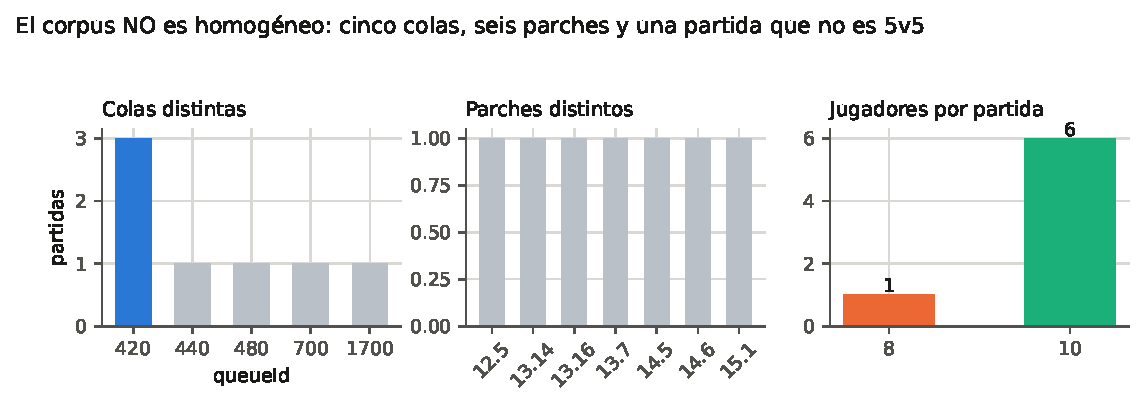
\includegraphics[width=\linewidth]{figuras/corpus.pdf}
  \caption{Composición del corpus. El panel derecho es el problema: una partida
  con 8 jugadores rompe el supuesto sobre el que se construye la métrica central.}
  \label{fig:corpus}
\end{figure}

\subsection{Campos opcionales: el payload cambia de forma dentro del mismo tipo}

\begin{table}[H]
\centering
\small
\caption{Campos opcionales por tipo de evento: la forma del payload cambia dentro del mismo tipo.}
\label{tab:opcionales}
\begin{tabular}{lrrrr}
\toprule
Evento & n & \% con position & \% con asistencias & Claves (mín--máx) \\
\midrule
CHAMPION\_KILL & 366 & 100.0 & 82.2 & 9--11 \\
BUILDING\_KILL & 90 & 100.0 & 47.8 & 8--10 \\
ELITE\_MONSTER\_KILL & 59 & 100.0 & 74.6 & 7--9 \\
WARD\_PLACED & 1332 & 0.0 & 0.0 & 4--4 \\
ITEM\_PURCHASED & 1404 & 0.0 & 0.0 & 4--4 \\
\bottomrule
\end{tabular}
\end{table}


Un JSON de la API no tiene columnas fijas. Dos eventos del mismo tipo pueden traer
distinto número de claves, y leerlos con acceso directo revienta:

\begin{itemize}[leftmargin=1.4em,itemsep=.25em]
  \item Sólo el \dato{9,1\,\%} de los 6\,877 eventos trae \texttt{position}. Decir
        «los eventos traen coordenadas» es falso como generalización: es cierto
        para asesinatos, estructuras y monstruos, y falso para compras de objeto,
        subidas de nivel y guardianes, que son la mayoría.
  \item \dato{65} de los \dato{366} \texttt{CHAMPION\_KILL} no traen
        \texttt{assistingParticipantIds}. No es un error: son los asesinatos en
        solitario. Y son justo los más informativos para la fase de línea, así que
        un \texttt{len()} directo se cae precisamente en los casos que interesan.
  \item \dato{3} asesinatos tienen \texttt{killerId} = 0: los ejecutó una torre o
        los súbditos. No hay equipo al que atribuirlos. \textbf{Qué haría:}
        tratarlos como una tercera categoría, no como del rival — que es lo que
        pasa si uno compara con \texttt{==} sin pensarlo.
\end{itemize}

\noindent \textbf{Regla práctica:} leer todo campo opcional con acceso defensivo y
reportar la tasa de ausencia de cada uno, no asumir el esquema.

\subsection{Duplicados y rangos}
No hay partidas repetidas (7 \texttt{matchId} únicos) ni cuadros duplicados. El
campo \texttt{frameInterval} midió \dato{60\,000\,ms} en las 7 de 7 partidas: un
cuadro por minuto exacto. Conviene subrayar que esto es un valor \emph{medido}, no
una garantía de la documentación — Riot no publica ese número, lo reporta cada
partida en su propio payload.

\begin{figure}[H]\centering
  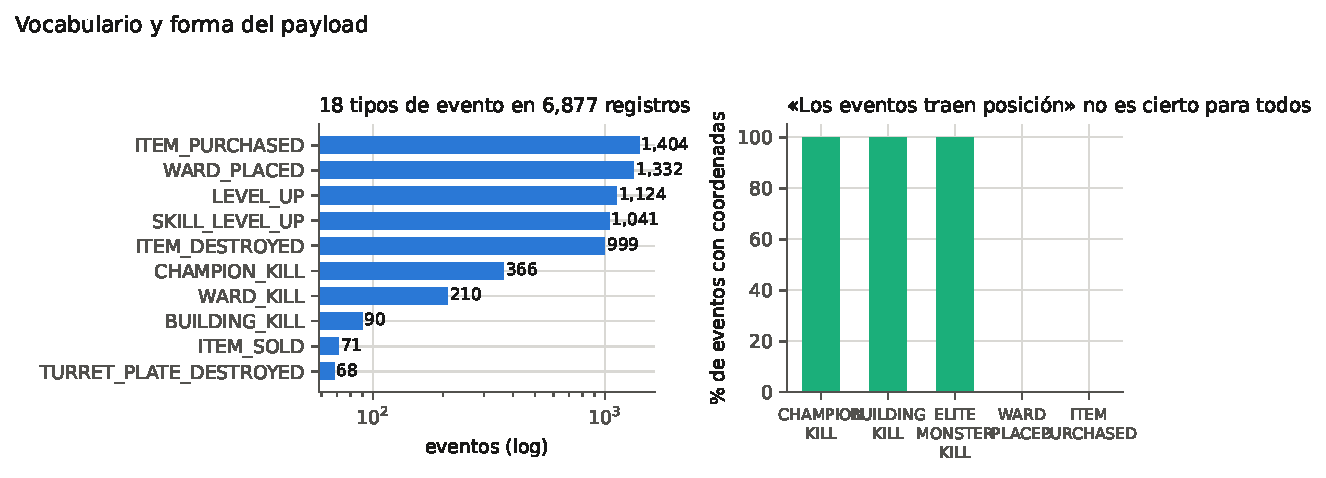
\includegraphics[width=\linewidth]{figuras/eventos.pdf}
  \caption{Los 18 tipos de evento observados y la proporción de cada uno que trae
  coordenadas.}
  \label{fig:eventos}
\end{figure}

% ===========================================================================
\section{Métricas básicas}

\begin{table}[H]
\centering
\small
\caption{Métricas por participante (68 filas).}
\label{tab:metricas}
\begin{tabular}{lrrrrrrr}
\toprule
Variable & n & media & desv. & varianza & mín & mediana & máx \\
\midrule
oro & 68.00 & 13006.78 & 3332.96 & 11108593.88 & 7308.00 & 12428.00 & 20500.00 \\
cs & 68.00 & 151.12 & 99.65 & 9931.00 & 0.00 & 165.50 & 324.00 \\
dano & 68.00 & 21243.94 & 11484.46 & 131892833.01 & 4253.00 & 18452.00 & 51538.00 \\
vision & 68.00 & 26.47 & 22.13 & 489.72 & 0.00 & 23.00 & 107.00 \\
k & 68.00 & 5.34 & 3.48 & 12.08 & 0.00 & 5.00 & 15.00 \\
d & 68.00 & 5.38 & 2.68 & 7.17 & 1.00 & 5.00 & 15.00 \\
a & 68.00 & 7.88 & 5.26 & 27.63 & 0.00 & 7.00 & 23.00 \\
nivel & 68.00 & 15.47 & 1.79 & 3.21 & 12.00 & 16.00 & 18.00 \\
\bottomrule
\end{tabular}
\end{table}


\begin{figure}[H]\centering
  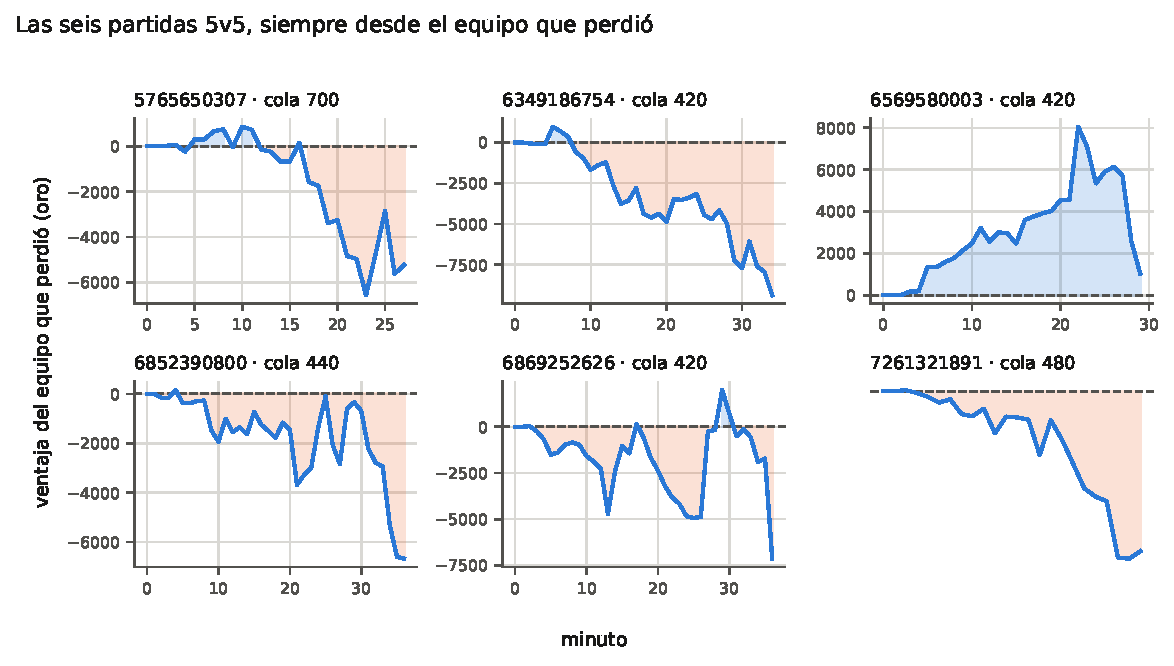
\includegraphics[width=\linewidth]{figuras/curvas.pdf}
  \caption{La variable central del proyecto: diferencia de oro por minuto, en las
  seis partidas 5v5, siempre vista desde el equipo que terminó perdiendo. Azul es
  ventaja; naranja, desventaja.}
  \label{fig:curvas}
\end{figure}

La figura~\ref{fig:curvas} es el objeto de estudio del proyecto. Se ve de
inmediato que las seis derrotas no tienen la misma forma: unas empiezan abajo y no
se recuperan, otras van arriba casi todo el tiempo. Ésa es precisamente la
observación que justifica clasificar las derrotas por su forma en vez de resumirlas
con un promedio.

% ===========================================================================
\section{Hipótesis y qué se puede probar aquí}

El proyecto declara seis hipótesis. Este corpus piloto no puede contrastar
ninguna —son 6 partidas 5v5, de las cuales 3 en la cola correcta— pero sí puede
responder algo más urgente: \textbf{¿es siquiera construible la variable con la
que están escritas?} Ésa es la pregunta que un piloto contesta.

\begin{enumerate}[leftmargin=1.6em,itemsep=.35em]
  \item \textbf{Se puede construir la diferencia de oro por minuto.} Sí, agregando
        \texttt{cuadros} — pero no es un campo de la API, y en la partida de Arena
        el cálculo da un número falso sin avisar.
  \item \textbf{Se pueden ubicar los objetivos en el tiempo.} Sí:
        \texttt{ELITE\_MONSTER\_KILL} y \texttt{BUILDING\_KILL} traen equipo y
        marca de tiempo en las 6 partidas.
  \item \textbf{El signo de la diferencia de oro informa sobre el resultado.} Sí,
        pero no desde el principio — ver la sección de señal.
  \item \textbf{Las reglas de arquetipo son aplicables mecánicamente.} Sí, y el
        resultado es incómodo: dejan la mitad sin clasificar (sección~\ref{sec:arq}).
\end{enumerate}

% ===========================================================================
\section{Varianza}

\begin{table}[H]
\centering
\small
\caption{Varianza antes y después de normalizar (grano: participante).}
\label{tab:varianza}
\begin{tabular}{lrrr}
\toprule
Variable & Varianza cruda & z-score & min--max \\
\midrule
participantId & 8.120 & 1.000 & 0.1003 \\
oro & 11,108,593.876 & 1.000 & 0.0638 \\
dano & 131,892,833.011 & 1.000 & 0.0590 \\
cs & 9,931.001 & 1.000 & 0.0946 \\
vision & 489.716 & 1.000 & 0.0428 \\
nivel & 3.208 & 1.000 & 0.0891 \\
k & 12.078 & 1.000 & 0.0537 \\
d & 7.165 & 1.000 & 0.0366 \\
a & 27.628 & 1.000 & 0.0522 \\
gano & 0.254 & 1.000 & 0.2537 \\
\bottomrule
\end{tabular}
\end{table}


\begin{figure}[H]\centering
  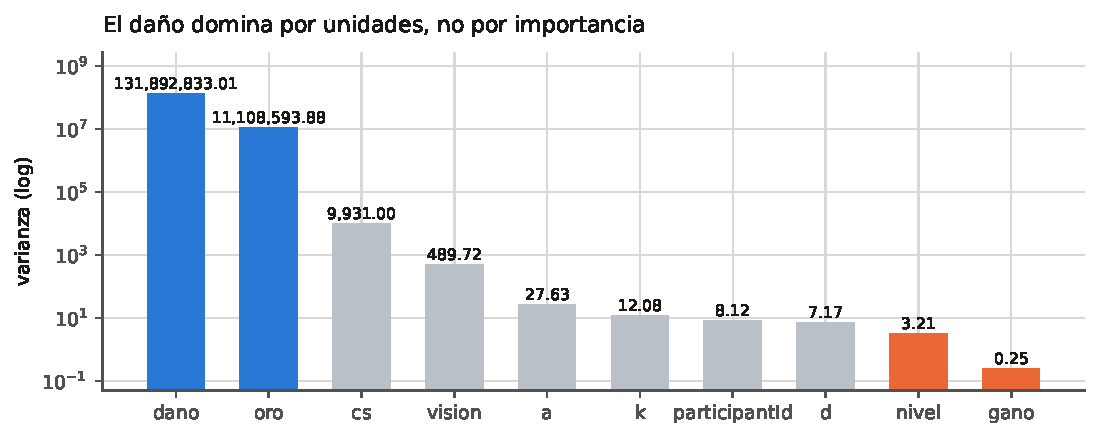
\includegraphics[width=\linewidth]{figuras/varianza.pdf}
  \caption{Varianza por variable, grano participante, en escala logarítmica.}
  \label{fig:var}
\end{figure}

\subsection{Las dos de mayor y las dos de menor varianza}

\begin{respuesta}{Mayor: \texttt{dano} (131\,892\,833) y \texttt{oro} (11\,108\,594). Menor: \texttt{gano} (0,254) y \texttt{nivel} (3,21)}
Y otra vez la varianza no dice nada sobre utilidad: \texttt{dano} encabeza la lista
porque se mide en unidades de daño, que llegan a decenas de miles. \texttt{gano} es
la variable objetivo y es la de menor varianza de todas.
\end{respuesta}

\noindent El caso de \texttt{gano} tiene una particularidad bonita que el Titanic
no tiene: en un 5v5 \emph{exactamente} la mitad de los participantes gana, por
construcción. Su proporción es 0,5 casi por definición y su varianza es
\(p(1-p)\approx 0{,}25\) — el máximo posible para una variable binaria. Es decir,
es la variable más «equilibrada» del conjunto y aun así la de menor varianza
absoluta, porque la varianza depende de la escala y una binaria vive entre 0 y 1.

\subsection{¿Conviene mucha o poca varianza?}

\begin{respuesta}{Ni una ni otra; y en este conjunto la trampa es aún más clara que en el Titanic}
\texttt{dano} tiene una varianza \textbf{519 millones de veces} mayor que
\texttt{gano}, y no es 519 millones de veces más informativa: está medida en otra
unidad. Sólo la varianza cero descalifica a una variable. Lo que informa es cuánto
se separa la variable entre las clases que se quieren distinguir, no cuánto se
dispersa en total.
\end{respuesta}

\subsection{¿Normalizar afecta la varianza?}

\begin{respuesta}{Sí. Con z-score las diez variables quedan en 1,000 exacto}
\end{respuesta}

\noindent Con min--max quedan todas entre 0 y 1 pero desiguales, y el orden se
invierte por completo: \texttt{gano} pasa a ser la de \emph{mayor} varianza
(\dato{0,2537}) y \texttt{d} la de menor (\dato{0,0366}). La razón es la misma que
en cualquier conjunto con colas largas: min--max divide entre el rango, y el rango
de \texttt{dano} lo fija un solo jugador con una partida excepcional.

Para este proyecto la consecuencia es concreta: cualquier agrupamiento de partidas
por forma de la curva tiene que normalizarse antes, o el resultado lo decidirá la
escala del oro y no la forma.

\begin{figure}[H]\centering
  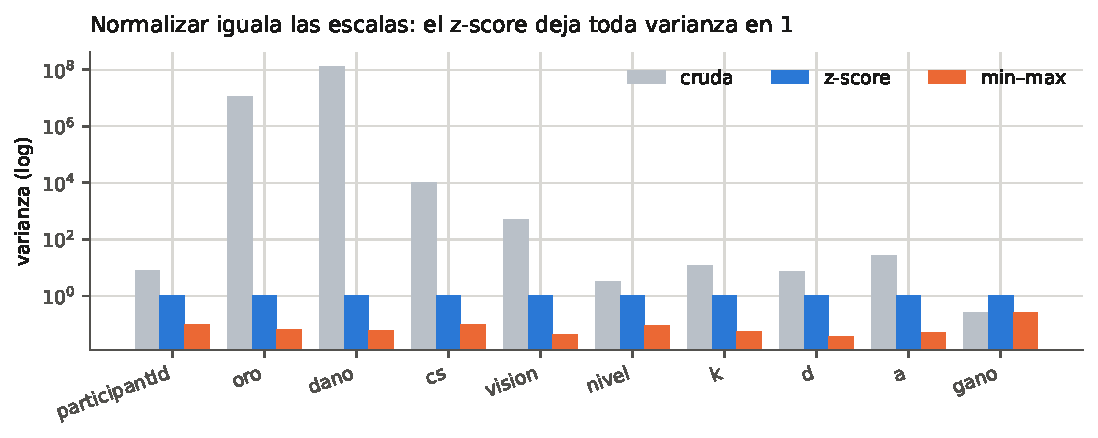
\includegraphics[width=\linewidth]{figuras/normalizacion.pdf}
  \caption{Varianza cruda, con z-score y con min--max.}
  \label{fig:norm}
\end{figure}

% ===========================================================================
\section{Distribuciones muestrales}

\begin{figure}[H]\centering
  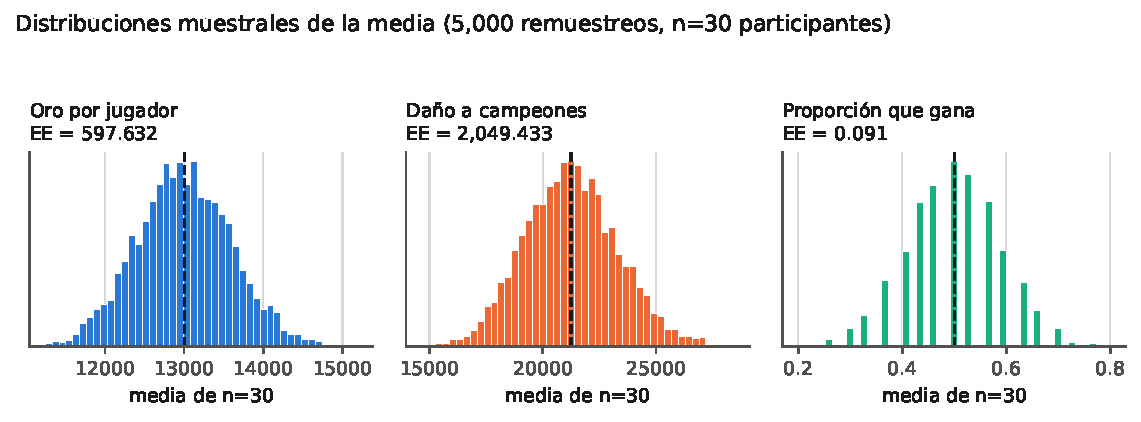
\includegraphics[width=\linewidth]{figuras/sampling.pdf}
  \caption{Distribuciones muestrales de la media, 5\,000 remuestreos de \(n=30\)
  participantes.}
  \label{fig:sampling}
\end{figure}

\begin{table}[H]\centering\small
\caption{Distribución muestral de la media, \(n=30\), 5\,000 remuestreos.}
\label{tab:sampling}
\begin{tabular}{lrrl}
\toprule
Variable & Media & Error estándar & IC 95\,\% \\
\midrule
Oro por jugador & 13\,001,66 & 597,63 & [11\,841,66 ; 14\,190,26] \\
Daño a campeones & 21\,255,89 & 2\,049,43 & [17\,437,50 ; 25\,373,09] \\
Proporción que gana & 0,501 & 0,091 & [0,33 ; 0,67] \\
\bottomrule
\end{tabular}
\end{table}

El renglón que enseña algo es el tercero. Sabemos con certeza matemática que la
proporción real de ganadores es \(0{,}5\) —es un 5v5— y aun así una muestra de 30
participantes la estima en un intervalo de \dato{[0,33 ; 0,67]}, 34 puntos de
ancho. Sirve como calibración honesta: si con una cantidad \emph{conocida} el
intervalo es así de ancho a \(n=30\), conviene desconfiar de cualquier porcentaje
que el proyecto reporte sobre unas pocas decenas de derrotas.

% ===========================================================================
\section{¿Cuánto ruido tiene el conjunto?}

En este proyecto el «ruido» no es un error de captura: es cuánto de una partida no
está determinado por lo observable en un momento dado. Una forma directa de
medirlo es preguntar, minuto a minuto, si el signo de la diferencia de oro coincide
con el resultado final.

\begin{figure}[H]\centering
  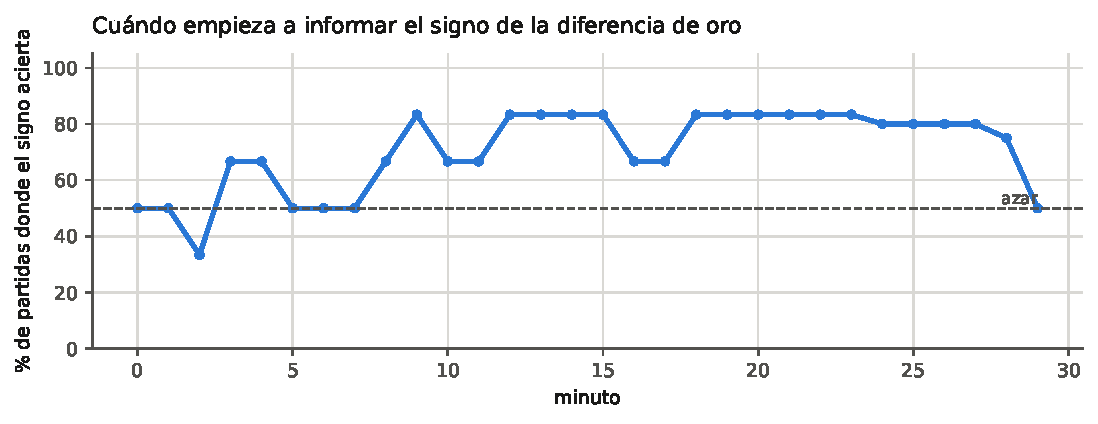
\includegraphics[width=\linewidth]{figuras/senal.pdf}
  \caption{Porcentaje de partidas en las que el equipo con más oro en ese minuto
  terminó ganando.}
  \label{fig:senal}
\end{figure}

\begin{respuesta}{En el minuto 5 el oro no informa nada: acierta el 50\,\%, exactamente el azar}
Sube a \dato{67\,\%} en el minuto 10 y a \dato{83\,\%} en el 15, donde se estanca.
\end{respuesta}

\noindent Tres lecturas, con su advertencia:

\begin{enumerate}[leftmargin=1.6em,itemsep=.3em]
  \item El \dato{50\,\%} del minuto 5 es el dato más útil del piloto: confirma que
        la ventana temprana es esencialmente ruido, y que el proyecto tiene que
        mirar la \emph{evolución} de la ventaja y no su valor en un instante.
  \item El estancamiento en \dato{83\,\%} a partir del minuto 15 sugiere que hay
        un residuo que el oro no explica — que es, precisamente, lo que el proyecto
        quiere caracterizar con los arquetipos.
  \item La ligera caída a \dato{80\,\%} en el minuto 25 \textbf{no significa
        nada}: con seis partidas, una sola cambia el porcentaje 17 puntos. Se
        reporta para no seleccionar sólo lo que confirma.
\end{enumerate}

\noindent \textbf{Advertencia grande:} estos porcentajes se calculan sobre
\dato{6} partidas. No son una estimación del ruido de League of Legends; son la
demostración de que la medida se puede calcular y de que su forma tiene sentido.
Con la muestra real habrá que reportarlos con intervalos de Wilson.

% ===========================================================================
\section{Las reglas de arquetipo, puestas a prueba}
\label{sec:arq}

El proyecto propone clasificar cada derrota en cuatro arquetipos con reglas de
umbral fijadas por escrito antes de ver los datos. La medida base es
\[
  v(t) \;=\; \frac{\text{diferencia de oro del equipo}}{\text{oro total de los diez jugadores}}
\]
con \emph{ventaja real} definida como \(v \ge 5\)\,\% y al menos 1\,500 de oro, y
\emph{decisiva} como \(|v| \ge 10\)\,\%. Aplicar esas reglas al corpus es la única
prueba real que un piloto puede hacer de ellas.

\begin{table}[H]
\centering
\small
\caption{Las reglas con umbral aplicadas a las seis partidas 5v5 del corpus.}
\label{tab:arquetipos}
\begin{tabular}{lrrr}
\toprule
matchId & cola & Racha con ventaja real (min) & Arquetipo \\
\midrule
EUW1\_5765650307 & 700 & 0 & A3 \\
EUW1\_6349186754 & 420 & 0 & A1 \\
EUW1\_6569580003 & 420 & 12 & A2 \\
EUW1\_6852390800 & 440 & 0 & sin clasificar \\
EUW1\_6869252626 & 420 & 0 & sin clasificar \\
EUW1\_7261321891 & 480 & 0 & sin clasificar \\
\bottomrule
\end{tabular}
\end{table}


\begin{figure}[H]\centering
  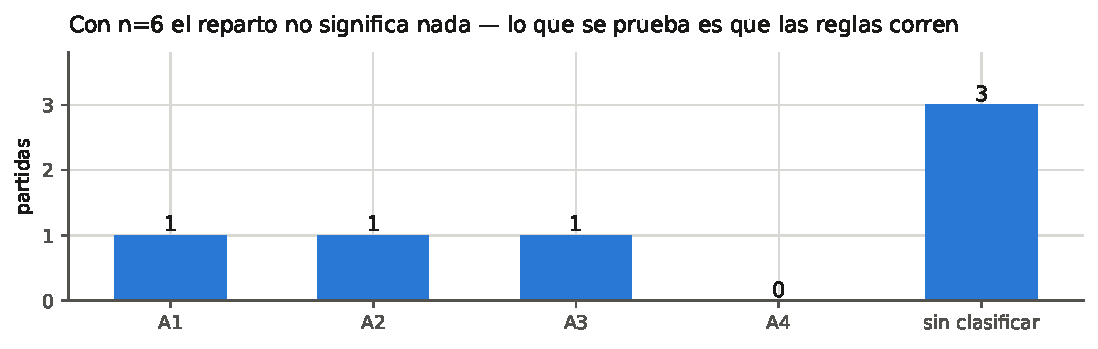
\includegraphics[width=\linewidth]{figuras/arquetipos.pdf}
  \caption{Resultado de aplicar las reglas publicadas a las seis partidas 5v5.}
  \label{fig:arq}
\end{figure}

\begin{respuesta}{Las reglas dejan 3 de 6 partidas sin clasificar}
Es el hallazgo más accionable del piloto, y va en contra de lo que uno querría
encontrar.
\end{respuesta}

\noindent Qué se aprende de esto, sin maquillarlo:

\begin{itemize}[leftmargin=1.4em,itemsep=.3em]
  \item Las reglas \textbf{corren mecánicamente} y son reproducibles: ése era el
        primer requisito y se cumple.
  \item La partida que la presentación usa como ejemplo (\texttt{EUW1\_6569580003})
        cae en \textbf{A2}, «ventaja temprana desperdiciada», que es exactamente lo
        que la presentación afirma. Las reglas y el relato no se contradicen.
  \item Pero un residuo del \dato{50\,\%} es demasiado alto para ser útil. Con la
        muestra real hay dos salidas honestas: ensanchar las bandas, o aceptar que
        el residuo es grande y reportarlo como resultado en vez de esconderlo
        forzando cada partida dentro de una caja.
  \item Lo que \emph{no} se puede hacer es ajustar los umbrales hasta que el
        residuo desaparezca. Un conjunto de reglas que clasifica el 100\,\% de las
        partidas es la señal de que se ajustaron después de ver los datos.
\end{itemize}

\noindent Con 6 partidas, «la mitad sin clasificar» tiene un intervalo enorme y no
es una estimación del residuo real. Es una alerta temprana, que es justo para lo
que sirve un piloto.

% ===========================================================================
\section{Respuestas concentradas}

\begin{longtable}{p{6.4cm}p{8.6cm}}
\caption{Las preguntas de la actividad, respondidas sobre este corpus.}\\
\toprule
\textbf{Pregunta} & \textbf{Respuesta} \\
\midrule
\endfirsthead
\toprule
\textbf{Pregunta} & \textbf{Respuesta} \\
\midrule
\endhead
¿Cuánto ruido puede llegar a tener el conjunto? &
En el minuto 5 el signo del oro acierta el 50\,\% — azar puro. Sube a 67\,\% en el
10 y se estanca en 83\,\% desde el 15. Ese 17\,\% que no explica el oro es el
espacio donde vive la pregunta del proyecto. Medido sobre 6 partidas. \\
\addlinespace
¿Qué variables tienen valores únicos y no sirven en un clasificador? &
\texttt{matchId} (7 de 7), \texttt{puuid} y los nombres de invocador (uno por
jugador). Además \texttt{participantId} es un índice de 1 a 10 sin contenido:
tiene varianza (8,12) y valor predictivo cero. \\
\addlinespace
¿Cuáles son categóricas y cuáles numéricas? &
Numéricas continuas: \texttt{oro}, \texttt{dano}, \texttt{xp}. Discretas:
\texttt{k}, \texttt{d}, \texttt{a}, \texttt{cs}, \texttt{nivel}, \texttt{vision}.
Categóricas nominales: \texttt{campeon}, \texttt{rol}, \texttt{tipo} de evento,
\texttt{teamId}, \texttt{cola}. Binaria: \texttt{gano}. Temporal: \texttt{minuto},
\texttt{timestamp}. \\
\addlinespace
Las dos variables con mayor varianza &
\texttt{dano} (131\,892\,833) y \texttt{oro} (11\,108\,594) —
ambas por sus unidades, no por su importancia. \\
\addlinespace
Las dos variables con menor varianza &
\texttt{gano} (0,254) y \texttt{nivel} (3,21). La primera es el objetivo. \\
\addlinespace
¿Son mejores las variables con mucha o poca varianza? &
Ninguna de las dos. \texttt{dano} tiene 519 millones de veces la varianza de
\texttt{gano} y no es más informativa: está en otra unidad. Sólo la varianza cero
descalifica. \\
\addlinespace
Si normalizamos, ¿se ve afectada la varianza? &
Sí. Con z-score las diez quedan en 1,000 exacto. Con min--max el orden se invierte:
\texttt{gano} pasa a ser la de mayor varianza (0,2537) y \texttt{d} la de menor
(0,0366). \\
\bottomrule
\end{longtable}

% ===========================================================================
\section{Conclusiones}

\begin{enumerate}[leftmargin=1.6em,itemsep=.4em]
  \item \textbf{El canal de datos funciona.} De siete pares de JSON anidados se
        derivan cuatro tablas limpias con 8\,999 filas en total, y la variable
        central del proyecto —la diferencia de oro por minuto— se puede construir.
  \item \textbf{El corpus obliga a filtrar antes de analizar.} Una partida de las
        siete no es 5v5 y el cálculo de oro habría dado un número falso sin fallar.
        Pedir \texttt{queue=420} explícito no es un detalle: es lo que evita ese
        error.
  \item \textbf{El esquema no es fijo.} Sólo el 9,1\,\% de los eventos trae
        coordenadas y el 18\,\% de los asesinatos no trae lista de asistencias.
        Todo campo opcional se lee con acceso defensivo.
  \item \textbf{La ventana temprana es ruido.} El oro del minuto 5 no informa
        nada. Eso valida la decisión de estudiar la evolución de la ventaja y no
        su valor en un instante.
  \item \textbf{Las reglas de arquetipo corren, pero dejan la mitad fuera.} Es el
        resultado que hay que llevarse: sirve para ajustar el diseño ahora, antes
        de descargar la muestra real, que es exactamente para lo que existe un
        piloto.
\end{enumerate}

% ===========================================================================
\section*{Fuente de los datos}
\addcontentsline{toc}{section}{Fuente de los datos}

\noindent\textbf{Fuente:} ejemplos públicos de respuestas de \texttt{match-v5} del
repositorio \texttt{MingweiSamuel/riotapi-schema}. Sin llave de API y sin datos
personales: los nombres de invocador de los otros jugadores no se usan en ninguna
parte de este documento.

\vspace{.5cm}
\noindent{\small\color{suave} Este proyecto no está avalado por Riot Games y no
refleja las opiniones de Riot Games ni de nadie involucrado oficialmente en la
producción o administración de League of Legends. League of Legends y Riot Games
son marcas registradas de Riot Games,~Inc.}

\end{document}
